%% This is a Latex template file for articles submitted to
%% Comptes Rendus. Mathématique.
%% It uses the cedram.cls class file, which is available at
%% http://www.centre-mersenne.org/texmf 
%
%%  The following template indicates the main features of the class file.
%%  In order to avoid mistakes in the handling of metadata (name, title, etc.),
%%  please use all the commands (and only those) indicated in the preamble for
%%  the title and authors.

%% If your paper uses non-ascii characters, be aware that the class
%% uses ISO-Latin-1 by default (inputenc is already loaded). You can
%% opt for UTF-8 encoding using the Unicode documentclass option as
%% below. In this case, you must add the following line at the top of 
%% the  bibtex file 
%-*-coding: utf-8

%% English is the default language. You may use the `francais' class
%% option if the main language of your paper is French, you may provide an
%% Abridged version in the other language as a first unnumbered
%% section (see below).

\documentclass[CRMATH,Unicode,manuscript]{cedram}

%% Authors may use other style files (e.g. to create figures), as long as
%% they do not alter the layout of the article.
% \usepackage[all]{xypic}

%% Notice that the class and the configuration file for this journal
%% already load the following packages (don't load any conflicting
%% package like enumerate for modifying lists, or changing fonts, e.g.!)
%% enumerate, textcomp, amssymb, caption, graphicx, xcolor, array, 
%% lastpage, etex, ifplatform, amsfonts, hyperref, placeins, fontenc
%% (T1), fancyvrb.
%% In addition, this journal's style  relies on the Fourier-GUT font
%% that can be installed from CTAN. If you don't have them on your
%% computer, the file will compile but the layout will be adjusted in
%% production. 

%% Insert here your own symbols, as the following ones:
\newcommand{\bbR}{\mathbb{R}}
\newcommand{\bbC}{\mathbb{C}}
\newcommand{\bbZ}{\mathbb{Z}}


%% Title of the article. 
%% The optional argument [] is the short version of the title (unused),
%% and the mandatory argument {} the title itself
\title{An Upper Bound on the Cardinality of a Minimum Feedback Vertex Set for Directed Graphs}


%% Authors, addresses and supports.
%% The optional argument is for shortened version appearing in the headings. Please
%% distinguish between first, middle and last names with the appropriate commands.
\author{\firstname{Philip} \middlename{N.} \lastname{Brown}\CDRorcid{0000-0003-3953-0503}}
\address{University of Colorado Colorado Springs\\
1420 Austin Bluffs Parkway\\
CO Springs, CO 80918 USA}
%% Support for the first author 
% \thanks{}
\email[P. Brown]{philip.brown@uccs.edu}
%
%% Each \address command increments a counter. If you want to refer to an address already
%%  listed for a previous author, use the command below in lieu of \address. 
%% The number is the appearance order of that address (among all addresses)
% \addressSameAs{1}{<repeat address 1>}
% This can be done multiple times
%\addressSameAs{1}{Road to the 5th problem avenue, Germany}
%\addressSameAs{2}{Center for experimental machines, United Kingdom}

%% The grant number can be inserted in the database
%% This won't be printed. It should be acknowledged in \thanks as above.
% \CDRGrant[UKRC]{2019-$$55900}


%% If you want to inform the reader of the paper about your
%% supplementary material, you can refer to it this way. The file
%% itself should be placed in a directory called Attach.

%\ESM{Supplementary material for this article is supplied as a separate 
%archive available from  the journal's
%website under 
%%% this will be replaced by the DOI of the article
%article's URL 
%%\printDOI\ 
%or from the author.}

%% If yo have supplementary material, you have to declare it this way (the
%% file will be copied and linked on the website
%% PDF is the default file type
% \CDRsupplementaryTwotypes{supplementary-material}{\cdrattach{supplement-doc.pdf}}
%% For another file type you should declare the mime-type
% \CDRsupplementaryTwotypes[application/zip]{supplementary-material}{\cdrattach{mycode.zip}}


%% Keywords
\keywords{Directed Graphs, Minimum Feedback Vertex Set}


%% Mathematical classification (2010)
\subjclass{05C69}

%% Abstract should be placed before \maketitle (and, in fact, before
%% \begin{document is best)
\begin{abstract} 
We derive an upper bound on the cardinality of a minimum feedback vertex set for arbitrary directed graphs, and provide example graphs which achieve this bound.
\end{abstract}


%% If the paper is in English, you may provide French metadata
%% (alttitle, altabstract, altkeywords)
%% If the paper is in French, you must provide English metadata
%% (alttitle, altabstract, altkeywords)

\begin{document}


% Use the \maketitle command after the abstract
\maketitle


%% Beginning of text
%% Abridged versions
%% 1. English one if the paper is in French
% \selectlanguage{english}
% \section*{Abridged English version}
% <your text here>
% \selectlanguage{french}
% to go back to main language.

%%% 2. French one if the paper is in English
% \selectlanguage{french}
% \section*{Version française abrégée}
%Nous serons brefs.
%\selectlanguage{english}
%%to go back to main language.

% Example of section

Let $G=(V,E)$ be a directed, not necessarily connected graph.
%A \emph{directed cycle} in $G$ is a sequence of distinct vertices $\{e_1,\dots,e_i\}\subseteq E$ such that 
A subset of vertices $M\subseteq V$ is called a \emph{minimum feedback vertex set} if the subgraph induced by the removal of $M$ from $G$ contains no directed cycles and $M$ is the smallest such set of vertices.
The problem of finding a minimum feedback vertex set in an arbitrary graph is known to be NP-hard even in sparse graphs~\cite{Fomin2006,Borradaile2019} and its decision version was one of Karp's original 21 NP-complete problems~\cite{Karp1972}.
Nonetheless, identifying minimum feedback vertex sets in directed graphs has applications in a number of disparate domains, including deadlock recovery in operating systems and computer engineering~\cite{Lin2000}, and determining the inefficiency of Nash equilibria in game theory~\cite{Brown2019c}.


Recent years have seen considerable attention focused on deriving bounds on the cardinality of the minimum feedback vertex set for undirected graphs. For instance see bounds for planar graphs~\cite{Kelly2017}, hypercubes~\cite{Madelaine2008}, shuffles~\cite{Kralovic2003}, and further conjectures~\cite{Kowalik2010}.
However, there seems to be a lack of similar results for the valuable case of directed graphs.
Accordingly, this note presents a simple upper bound for this quantity for directed graphs as a function of the number of nodes and edges.
We present graphs that achieve this bound.
While tight in general, this bound can almost certainly be improved on specific classes of graphs, and we invite improvements from the mathematical community.

\section{Preliminaries}
We present the following definitions to ensure our results are clear.
A directed graph $G=(V,E)$ (or \emph{digraph}) is specified by vertex set $V$ and edge set $E$ and we assume that $G$ is simple (i.e., we forbid repeated edges or self-loops), but we do not require that $G$ is connected.
A \emph{directed cycle} is a sequence of distinct edges $\{e_1,e_2,\ldots,e_m\}$ and a corresponding sequence of distinct vertices $\{v_1,v_2,\ldots,v_m\}$ such that for all $i<m$, $e_i=(v_i,v_{i+1})$ and $e_m=(v_m,v_1)$.
Note that a directed cycle can have length 2; i.e., the graph $(\{v_1,v_2\},\{(v_1,v_2),(v_2,v_1)\})$ has a directed cycle.
A digraph $G$ is called \emph{acyclic} if if it contains no directed cycles.
A set of vertices $M\subseteq V$ is called a \emph{feedback vertex set} if the graph $\left(V\setminus M,E\setminus \{(i,j)\in E\ |\ i\in M \mbox{ or } j\in M\}\right)$ is acyclic.
The set $M$ is called a \emph{minimum feedback vertex set} if it is a feedback vertex set of minimum cardinality. 
We write $\alpha(G)$ to denote the cardinality of a minimum feedback vertex set for digraph $G$.

\section{Contribution}


Our main result gives a tight upper bound for all (not necessarily connected) digraphs as a function of the number of edges.
\begin{theo}\label{thm:main}
Let $G=(V,E)$ be a digraph.
Then
\begin{equation}\label{eq:main}
\alpha(G) \leq \min\left\{|V|-1,\left\lfloor\frac{|E|}{2}\right\rfloor\right\}.
\end{equation}
There exist graphs which achieve this bound.
\end{theo}

\begin{proof}
First we show the edge-based upper bound.
Let $G$ be a directed graph, and let $M(G)$ be a minimum feedback vertex set of $G$.
We wish to show that 
\begin{equation}
2\alpha(G)\leq |E|.
\end{equation}
Enumerate the $m$ vertices in $M(G):=\{u_1,u_2,\ldots,u_m\}$.
%Define $E(M(G)):=\{
Define the sequence $\{G_i\}_{i=0}^m$ as follows: $G_0=G$, and $G_i$ is the digraph that results from the removal of $u_i$ and all incident edges from $G_{i-1}$.
By the definition of $M(G)$, each vertex $u_i$ is contained in at least one cycle in graph $G_{i-1}$.
Since each $u_i$ is contained in a cycle in $G_{i-1}$, it follows that at least 2 edges are incident on $u_i$ in $G_{i-1}$.
Since the sequence of graphs satisfies $E(G_{i})\subset E(G_{i-1})$, this means that for all $i=1,\ldots,m$, at least 2 unique edges are incident on vertex $u_i$ which are \emph{not} incident on $u_j$ for any $j<i$.
%
Thus, writing $E(M(G))$ to denote the set of edges incident on $M(G)$, we have that
\begin{equation}
2\alpha(G)\leq|E(M(G))|\leq |E|.
\end{equation}

\begin{figure}[b]
\centering
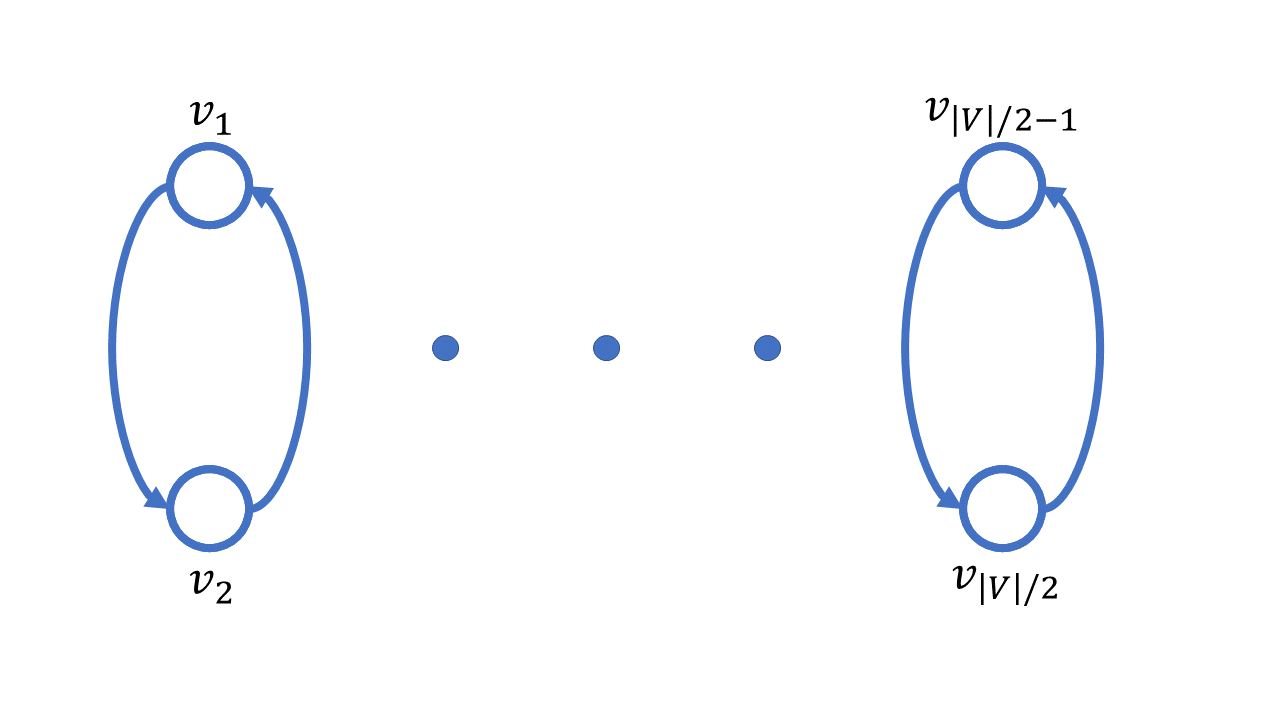
\includegraphics[width=.5\textwidth]{gfx/graph}
\caption{\label{fig:graph} Graph with $\alpha(G)=\lfloor|E|/2\rfloor$, achieving the bound given in Theorem~\ref{thm:main} in~\eqref{eq:main}.}
\end{figure}

To show the edge-based lower bound, we construct a family of graphs which satisfy~\eqref{eq:main} with equality for all $k$, where $|E|=k$.
Let $|V|=2\lfloor k/2\rfloor$, and let $E=\{(2i,2i-1)\cup(2i-1,2i)\ |\ i\in\{1,\ldots,|V|/2\}\}$ (see Figure~\ref{fig:graph}).
If $|E|$ is odd, define the single remaining edge between any feasible pair of vertices (e.g., $(1,3)$).
Since this graph contains exactly $|V|/2$ disjoint length-2 directed cycles, the cardinality of any minimum feedback vertex set is exactly $|V|/2$ (e.g., the set of odd-numbered vertices is such a set).
%


The vertex-based upper bound is trivial, since if $|V|-1$ vertices and associated edges are removed from any graph, the resulting graph is a single vertex and thus acyclic.
The vertex-based lower bound is achieved by a complete digraph.
\end{proof}




% The next command determines the bibliography style. Please do not
% change this.
\bibliographystyle{crplain}

%This calls all references from the .bib
%\nocite{*}

%  This inserts the bib file
\bibliography{../../library/library}


\end{document}










